\documentclass[10pt,a4paper]{report}
\usepackage[latin1]{inputenc}
\usepackage{amsmath}
\usepackage{amsfonts}
\usepackage{color}
\usepackage{amssymb}
\usepackage{graphicx}
\usepackage{fancyhdr}
\lhead{Introduction to \\ Computer Graphics}
\chead{Exercise number}
\rhead{Kevin Serrano, 204141 \\ Gianni Scarnera, 195899}
\pagestyle{fancy}
\author{Kevin Serrano, Gianni Scarnera}
\title{Exercise 2}
\begin{document}
\maketitle

\section*{2.1.1   Normals and Materials}
To get the material and the normal at the intersection point with the plane is very easy because the plan is a flat and infinite so the normal is the same everywhere on the plane. So to get the normal at the intersection we can use $iData\rightarrow normal = getNormal()$ and for the material : $iData\rightarrow material = getMaterial()$.


For the triangle is a little bit complicated because we have to interpolate the normals of vertices to get the normal at the intersection.
\begin{figure}[h!]
\caption{Normals of vertices and the interpolation at point q}
  \centering
    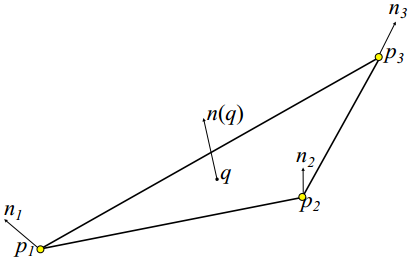
\includegraphics[width=0.5\textwidth]{triangleNormals.png}
\end{figure}

It's easy to interpolate the normal $n(q)$at a point $q$ inside the triangle with barycentric coordinates.
We can take our 3 values $s_1, s_2, s_3$ at point $q$ with the formulas of precedent exercise to compute the normal at point $q$ and normalized.
$$n(q) =  \frac{s_1 \mathbf{n_1} + s_2 \mathbf{n_2} + s_3 \mathbf{n_3}}{||s_1 \mathbf{n_1} + s_2 \mathbf{n_2} + s_3 \mathbf{n_3}|| }$$
where $\mathbf{n_1, n_2, n_3}$ are the normal at each vertices. Now we can get the normal and the material at the intersection of the triangle with $iData\rightarrow normal = n(q)$ and for the material : $iData\rightarrow material = getMaterial()$

\section*{2.1.2   Diffuse Lighting Model}
The diffuse reflection depends on surface orientation and light position but is independent of camera position. The brightness depends of the angle between the normal at intersection point and the source light.
\begin{figure}[h!]
\caption{angle between the normal (N) and the vector from intersection point to source light (L)}
  \centering
    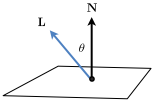
\includegraphics[width=0.3\textwidth]{angleNL.png}
\end{figure}
Now for each light in the scene, we have to compute the intensity at the intersection point with the diffuse formula $$I = I_p k_d cos(\theta) = I_p k_d (\mathbf{N \cdot{L}})$$ where $I_p$ is the color of the light source and $k_d$ the diffuse material color. To implement this formula, we have to take the vector of source light in the object $scene \rightarrow getLight()$ and then use a iterator to calculate the intensity $I$ of each light sources and then the resulting of different light sources are added up and clamped to [0,1] at the end. All vectors are normalized. Then after calculated and normalise the vector $L$ for each light source, we have to check if the light source and the normal point in the same direction, i.e $(\mathbf{N\cdot L}>0)$ otherwise the light does not contribute to diffuse shading. Then it's possible to calculate the intensity $I$ if we use the element-wise multiplication with $I_p$ and $k_d$ because they are Vector4. Then $I_p = lightsource \rightarrow getColor()$ and $k_d = iData \rightarrow material \rightarrow diffuse$
\begin{figure}[h!]
\caption{Diffuse shading model}
  \centering
    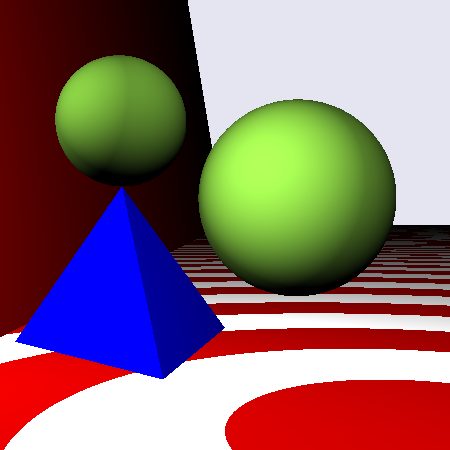
\includegraphics[width=0.5\textwidth]{02_Exc_Raytracing_Framework/Image_Diffuse_Model.png}
\end{figure}

\section*{2.1.3   Phong Lighting Model}
The phong lighting model is the combination of the ambient, diffuse and specular reflection.
\begin{figure}[h!]
\caption{Specular reflection}
  \centering
    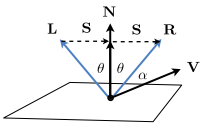
\includegraphics[width=0.3\textwidth]{angleRV.png}
\end{figure}
$\mathbf{L,N}$ are the same vector than before and $\mathbf{R}$ is the reflected vector from the light $\mathbf{L}$ with $\mathbf{N}$ with the same angle $\theta$, and $\mathbf{V}$ is the normalised vector from the intersection to the camera position.
So for each light source, we can calculate the vector $\mathbf{R}$ with the formula $$\mathbf{R} = 2 \mathbf{N} cos(\theta)-\mathbf{L} = ( 2 \bf N(N \cdot L)-L)$$
Then we can calculate the intensity of specular reflection for each light sources with the formula $$I_p k_s cos(\alpha)^n = I_p k_s (\mathbf{R \cdot V})^n$$ where $I_p$ is the color of the light, $k_s$ the specular color of the material, and $n$ the shininess of the material. So 
\begin{itemize}
\item $I_p = sourcelight \rightarrow getColor()$
\item $k_s = iData \rightarrow material \rightarrow specular$
\item $n = iData \rightarrow material \rightarrow shininess$
\end{itemize}
The intensity of the ambient is $I_{ambient} = I_a k_a$ where $I_a$ is the scene ambient light color, i.e $I_a = scene \rightarrow getAmbient()$ and $k_a$ is the ambient reflection color of the intersected objects material, i.e $k_a = iData \rightarrow material \rightarrow ambient$.
The intensity of the diffuse shading is $I_{diffuse}$ and it's the same formula as the part before.
Then we can add the intensity of the ambient, diffuse and specular reflection to get the Phong lighting Model $$ I = I_{ambient} + I_{diffuse} + I_{specular}$$ 
\begin{figure}[h!]
\caption{Phong lighting Model}
  \centering
    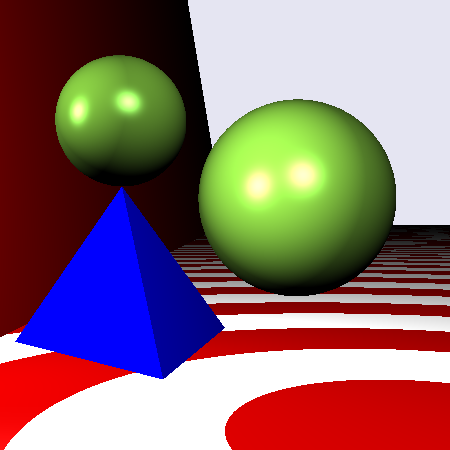
\includegraphics[width=0.5\textwidth]{02_Exc_Raytracing_Framework/2_1_3.png}
\end{figure}
\newpage

\section*{2.2.1   Shadows}
To create the shadows, we need to figure out for a point, which light are occluded and which are not. In the method getNonOccludedLights of Scene we retrieve the list of Lights not occluded for a selected point in the scene. To do so, for each Lights in the scene, we generate a ray from the point to the Light and we figure out with the method fastIntersect if this ray has an intersection in the scene or not. If not, then this Light is not occluded for the point and is added to the list. We then change the shade methods to use this method. Generateray sets maxt to avoid having a collision with the border of the point.
\begin{figure}[h!]
\caption{Shadows}
  \centering
    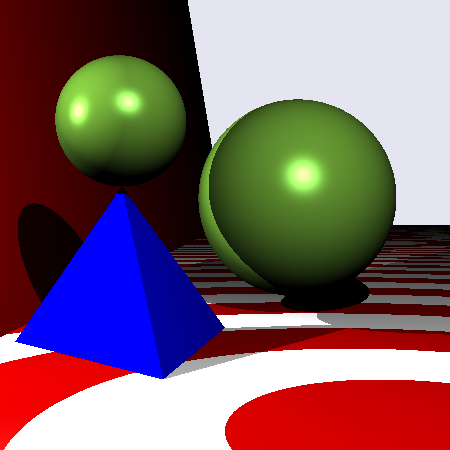
\includegraphics[width=0.5\textwidth]{02_Exc_Raytracing_Framework/2_2_1.png}
\end{figure}

\end{document}